\documentclass{article}
\usepackage{hyperref}


\usepackage{Sweave}
\begin{document}
\Sconcordance{concordance:hw3_R_joe_brew.tex:hw3_R_joe_brew.Rnw:%
1 4 1 1 0 2 1 1 27 15 1 1 41 1 2 19 1 1 6 5 0 1 1 1 4 1 0 1 18 17 0 1 3 %
1 0 3 1 1 3 1 0 1 1 3 0 1 2 7 1 1 2 27 0 1 2 6 1 1 2 1 0 2 1 11 0 1 2 3 %
1 1 2 1 0 2 1 11 0 1 2 11 1 1 8 6 0 1 2 1 0 1 6 4 0 1 2 1 0 1 5 3 0 1 5 %
3 0 1 6 4 0 1 5 3 0 2 1 3 0 2 2 20 0 1 2 6 1 1 5 4 0 1 5 3 0 1 6 7 0 1 %
2 1 5 4 0 1 1 1 3 2 0 1 4 3 0 1 6 5 0 1 7 9 0 1 2 8 1 1 2 16 0 1 2 3 1 %
1 5 4 0 1 3 1 0 1 3 1 0 1 4 3 0 1 3 1 0 5 1 3 0 1 2 2 1 1 17 15 0 1 3 6 %
0 1 1 5 0 1 1 5 0 1 1 5 0 1 1 5 0 1 1 9 0 1 3 3 1 1 2 1 0 1 1 1 2 1 0 1 %
4 3 0 1 5 3 0 1 6 4 0 1 2 1 0 1 2 1 0 1 2 1 0 1 2 1 0 1 2 1 0 1 2 1 0 1 %
8 11 0 1 3 2 1}



\begin{center}
\huge{HW 3: R supplement}\\
\large{Joe Brew}
\end{center}

\fbox{
  \parbox{\textwidth}{
    \noindent \textbf{Note to professor: } The following outlines the steps I've taken in R to replicate the tasks of HW 3.  Please note that I \emph{did not} follow all steps, since some are specific to ArcMap.  }
}\\

\noindent  \\

\noindent What follows is the output of the homework assignment (the two maps), followed by the code used to generate them.  Full code (including the code for this \LaTeX document) is available \href{https://github.com/joebrew/uf/tree/master/phc6194/hw3}{HERE}.

\begin{center}
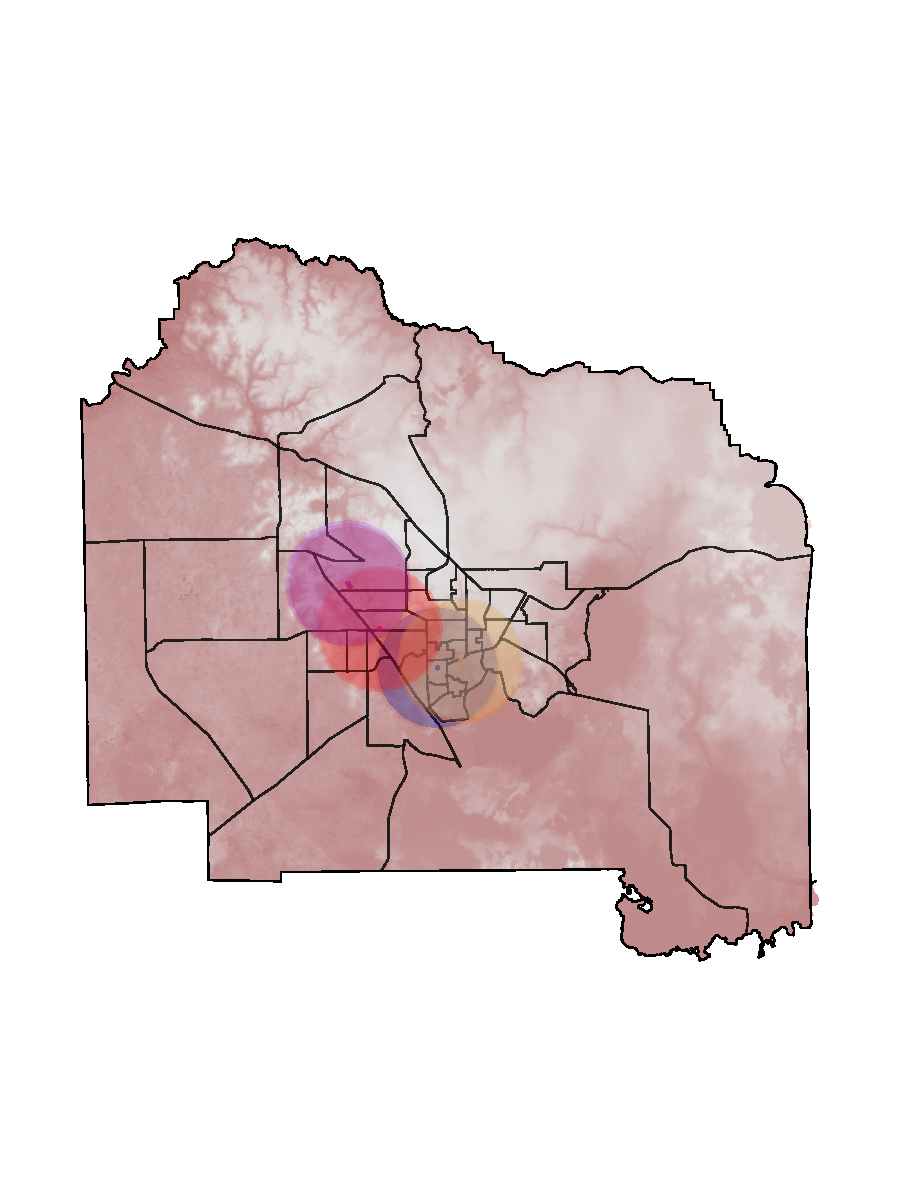
\includegraphics{hw3_R_joe_brew-002}
\end{center}

\newpage
\section*{Part 1}


\section*{Question 1}

Add the shapefile of "usa county" into ArcMap; Open the attribute table and select all records in FL (Please refer to "selecting records in a table" in the handout); Then export the selected record to create a new feature (i.e. Shapefile) of "CTY FL". \\

\noindent \textbf{NA}.  Since these data came in .dbf format (an ArcGIS proprietary format), I had to use Arc to export them to R. 

\section*{Question 2}

The dataset of "cancer fl.dbf" have the crude and age adjusted mortality rate in all counties in FL. Please join the cancer mortality data with the new shapefile of "CTY FL" that you create at step 1. Then, use the joined information to create a new shapefile with the cancer mortality information attached. (Note: please zip the Shapefile and submit it together with this word document for evaluation)


Given that the names of the cancer data and the county shape file didn't match up perfectly, I wrote some code that would find the "closest match" in order to make the merge.  See below:

\begin{center}
\begin{Schunk}
\begin{Sinput}
> #####
> # Fix names in the county shapefile and the cancer table
> # In order to make them compatible
> #####
> cancer$name <- as.character(toupper(gsub(" County, FL", "", cancer$County)))  
> county$name <- as.character(county$NAME2_)
> # Loop to find closest match
> cancer$newname <- NA
> for (i in 1:nrow(cancer)){
+   
+   #Create matrix of match scores
+   m <- adist(x = cancer$name[i],
+              y = county$name,
+              ignore.case = TRUE)
+   
+   #Select the index of the best (lowest) match
+   best <- which(m == min(m), arr.ind=TRUE)[1,]
+   best.ind <- as.numeric(best["col"])
+   #best.ind <- which.min(best)
+   
+   #Assign to best.num the actual score of the best match
+   best.num <- min(m)
+   
+   #Assign the best match to newad 
+   cancer$newname[i] <- as.character(county$name[best.ind])
+ }
> # See where matches weren't identical
> x <- cancer$name[which(cancer$name != cancer$newname)]
> y <- cancer$newname[which(cancer$name != cancer$newname)]
> cbind(x,y) # perfect
> rm(x,y)
> # Since the match is good, let's replace name with newname
> cancer$name <- cancer$newname
> cancer$newname <- NULL
\end{Sinput}
\end{Schunk}
\end{center}

%<<results = tex, print = TRUE>>=
%print(xtable(head(county), size = "\\tiny"))
%@

Here's what the resulting merged dataframe looks like:

\begin{Schunk}
\begin{Sinput}
> head(county)
\end{Sinput}
\begin{Soutput}
      name OBJECTID   ID_ NAME1_   NAME2_ PARTS_ POINTS_   LENGTH_     AREA_
0  ALACHUA      290 12001  12001  ALACHUA      1      24 134.10040  967.2103
1    BAKER      291 12003  12003    BAKER      1      14 107.51540  597.0373
2      BAY      292 12005  12005      BAY      1      15 143.36310  899.5897
3 BRADFORD      293 12007  12007 BRADFORD      1      12  86.15348  309.1252
4  BREVARD      294 12009  12009  BREVARD      1      20 184.24970 1316.7960
5  BROWARD      295 12011  12011  BROWARD      1       8 146.94380 1198.0390
  STATE_NAME STATE_ABBR Shape_Leng Shape_Area OID_              County
0    Florida         FL   2.093249 0.23289090   NA  Alachua County, FL
1    Florida         FL   1.668053 0.14476206   NA    Baker County, FL
2    Florida         FL   2.226471 0.21765530   NA      Bay County, FL
3    Florida         FL   1.330562 0.07469252   NA Bradford County, FL
4    Florida         FL   2.782362 0.31230985   NA  Brevard County, FL
5    Florida         FL   2.286041 0.27940666   NA  Broward County, FL
  County_cod Deaths Population Crude_Rate Age_Adjust
0      12001   1566     935112      167.5      198.4
1      12003    193      98959      195.0      225.5
2      12005   1475     646666      228.1      203.6
3      12007    248     112793      219.9      208.7
4      12009   6036    2107959      286.3      192.0
5      12011  14317    7016680      204.0      171.8
\end{Soutput}
\end{Schunk}


\section*{Question 3}
Using the shapefile created in step 2, please answer the following questions (Hint: Selection by attribute):

a.  Please find five top counties with the highest crude cancer mortality rate in Florida and list the information of county name and their rates below.

\begin{Schunk}
\begin{Sinput}
> county <- county[rev(order(county$Crude_Rate)),]
> x <- county[,c("name", "Crude_Rate")]
> print(data.frame(x[1:5,]))
\end{Sinput}
\begin{Soutput}
           name Crude_Rate
8        CITRUS      429.2
62        UNION      398.4
7     CHARLOTTE      369.6
26     HERNANDO      368.9
30 INDIAN RIVER      362.4
\end{Soutput}
\end{Schunk}


b.	Please find five top counties with the highest age-adjusted cancer mortality rates in Florida and also list the information of county name and their rates;

\begin{Schunk}
\begin{Sinput}
> county <- county[rev(order(county$Age_Adjust)),]
> x <- county[,c("name", "Age_Adjust")]
> print(data.frame(x[1:5,]))
\end{Sinput}
\begin{Soutput}
         name Age_Adjust
62      UNION      472.1
39    MADISON      253.1
66 WASHINGTON      248.1
23   HAMILTON      245.2
37       LEVY      242.3
\end{Soutput}
\end{Schunk}


c.	Please check if the selected five counties with highest crude and age-adjusted rates are same or different. If they are different, please explain why it is. \\

\noindent \textbf{NA}.  I answered this in the Arc assignment.

\newpage
\section*{Part 2}

\section*{Task 1} From the feature class of "FL Hospitals", please select all hospitals within Alachua County. (Hint: Using Alachua_boundary and "Intersect" tool). 
List the ID (FID FL Hospitals) and the names of the selected hospitals below for evaluation.

\begin{Schunk}
\begin{Sinput}
> #####
> # I FIRST EXPORTED THE LAYERS AS SHAPEFILES
> # FROM ARCGIS, NOW I READ THEM INTO R
> #####
> boundary <- readOGR("HW",
+                     layer = "Alachua_Boundary")
> hospitals <- readOGR("HW",
+                      layer = "FL_Hospitals")
> #####
> # Convert some objects to ned's projection
> #####
> hospitals2 <- spTransform(hospitals,
+                           CRS(proj4string(ned)))
> boundary2 <- spTransform(boundary,
+                          CRS(proj4string(ned)))
> #####
> # Create a rasterlayer version of ned
> #####
> rned <- raster(ned)
> #####
> # Create an image version of ned
> #####
> ined <- as.im(ned)
> #####
> # Use extract() to get the pixel values of the raster
> # version of ned at the locations of the hospitals
> #####
> hospitals2$elevation <- extract(rned, coordinates(hospitals2))
> #####
> # Keep only hospitals which are in Alachua's borders
> #####
> x <- over(hospitals2, polygons(boundary2))
> hospitals2 <- hospitals2[which(!is.na(x)),]
> rm(x)
\end{Sinput}
\end{Schunk}

\begin{Schunk}
\begin{Sinput}
> data.frame(hospitals2[,c("NAME", "ADDRESS", "CITY", "ZIPCODE")])
\end{Sinput}
\begin{Soutput}
                                      NAME                    ADDRESS
27 SELECT SPECIALTY HOSPITAL - GAINESVILLE          2708 SW ARCHER RD
28        MALCOM RANDALL VA MEDICAL CENTER        1601 SW ARCHER ROAD
29     SHANDS AT THE UNIVERSITY OF FLORIDA 1600 SOUTHWEST ARCHER ROAD
31   NORTH FLORIDA REGIONAL MEDICAL CENTER    6500 WEST NEWBERRY ROAD
32          SHANDS VISTA BEHAVIORAL HEALTH       4101 N.W. 89TH BLVD.
33                   SHANDS REHAB HOSPITAL     4101 NW 89TH BOULEVARD
          CITY ZIPCODE coords.x1 coords.x2
27 GAINESVILLE   32608  558186.8  626089.2
28 GAINESVILLE   32608  560032.9  626653.6
29 GAINESVILLE   32610  560096.6  626998.7
31 GAINESVILLE   32605  553520.9  629225.1
32 GAINESVILLE   32606  550977.8  632903.1
33 GAINESVILLE   32606  551139.2  632615.6
\end{Soutput}
\end{Schunk}



\section*{Task 2}

Find the elevation information for the selected hospitals in Alachua County using the data of "NED01".  List the ID (FID FL Hospitals) of the hospitals and their elevations for evaluation.

\begin{Schunk}
\begin{Sinput}
> #####
> # READ IN THE RASTER ELEVATION DATA
> #####
> ned <- readGDAL("HW/ned011.tif")
> #####
> # Create a rasterlayer version of ned
> #####
> rned <- raster(ned)
> #####
> # Use extract() to get the pixel values of the raster
> # version of ned at the locations of the hospitals
> #####
> hospitals2$elevation <- extract(rned, coordinates(hospitals2))
\end{Sinput}
\end{Schunk}

\begin{Schunk}
\begin{Sinput}
> #####
> # Define a color vector and plot the image of ned
> #####
> mycols <- colorRampPalette(c("blue", "darkgreen", "grey", "white"))(60)
> mycols <- adjustcolor(mycols, alpha.f=0.6)
> plot(ined,
+      col = mycols,
+      main = "Alachua hospitals and elevation")
> #Points
> points(hospitals2,
+        col = adjustcolor("darkred", alpha.f=0.6),
+        pch = 16)
> # Text
> text(x = coordinates(hospitals2)[,1],
+      y = coordinates(hospitals2)[,2],
+      labels = hospitals2$elevation, cex = 0.6,
+      col = adjustcolor("black", alpha.f=0.7),
+      pos = c(1,3))
> # Text (names)
> text(x = coordinates(hospitals2)[,1],
+      y = jitter(coordinates(hospitals2)[,2], factor = 4),
+      labels = hospitals2$NAME, cex = 0.3,
+      col = adjustcolor("black", alpha.f=0.4),
+      pos = 4)
\end{Sinput}
\end{Schunk}
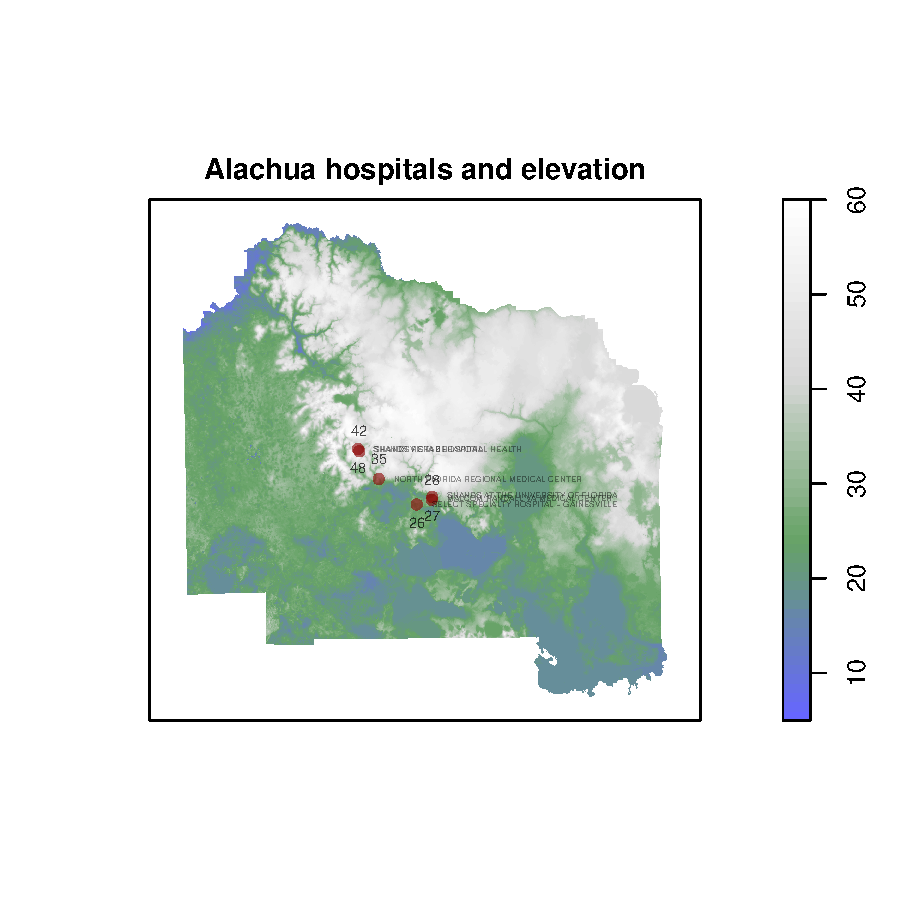
\includegraphics{hw3_R_joe_brew-010}

\section*{Task 3}


Find the serving population within 5km distance of each hospital using census tract population in Alachua. List the ID (FID FL Hospitals) of the hospitals and the number of the serving population within 5 km distance for evaluation.
 (Hint: Creating a buffer of 5 km for each hospital and then spatial join the census population using Spatial Join tool. Figure 1 shows how to assess the tool. In addition, in spatial join tool, right click the variables and you can select the statistics as shown in the second figure) \\
 
 First, I'll show you the answer.

% latex table generated in R 3.1.1 by xtable 1.7-3 package
% Mon Sep 22 17:29:45 2014
\begin{table}[ht]
\centering
\begin{tabular}{rll}
  \hline
 & Hospital & Population \\ 
  \hline
1 & SELECT SPECIALTY HOSPITAL - GAINESVILLE & 103513 \\ 
  2 & MALCOM RANDALL VA MEDICAL CENTER & 110464 \\ 
  3 & SHANDS AT THE UNIVERSITY OF FLORIDA & 120194 \\ 
  4 & NORTH FLORIDA REGIONAL MEDICAL CENTER & 95981 \\ 
  5 & SHANDS VISTA BEHAVIORAL HEALTH & 61276 \\ 
  6 & SHANDS REHAB HOSPITAL & 61276 \\ 
   \hline
\end{tabular}
\end{table}
[1] "% latex table generated in R 3.1.1 by xtable 1.7-3 package\n% Mon Sep 22 17:29:45 2014\n\\begin{table}[ht]\n\\centering\n\\begin{tabular}{rll}\n  \\hline\n & Hospital & Population \\\\ \n  \\hline\n1 & SELECT SPECIALTY HOSPITAL - GAINESVILLE & 103513 \\\\ \n  2 & MALCOM RANDALL VA MEDICAL CENTER & 110464 \\\\ \n  3 & SHANDS AT THE UNIVERSITY OF FLORIDA & 120194 \\\\ \n  4 & NORTH FLORIDA REGIONAL MEDICAL CENTER & 95981 \\\\ \n  5 & SHANDS VISTA BEHAVIORAL HEALTH & 61276 \\\\ \n  6 & SHANDS REHAB HOSPITAL & 61276 \\\\ \n   \\hline\n\\end{tabular}\n\\end{table}\n"
Now, I'll show you how I got it: \\
 
First, I created the buffer zones of 5 kilometers in all directions.
\begin{Schunk}
\begin{Sinput}
> #####
> # CREATE GEOGRAPHICAL BUFFER
> #####
> library(rgeos)
> # Check out the projection string of hospitals2 to confirm meters
> proj4string(hospitals2)
> # Create buffered shapefiles
> mylist <- list()
> for (i in 1:length(hospitals2$NAME)){
+   mylist[i] <- 
+     gBuffer(hospitals2[which(hospitals2$NAME == hospitals2$NAME[i]),], width = 5000)
+ }
> # Unlist each hospital into its own object
> hosp1 <- unlist(mylist[[1]])
> hosp2 <- unlist(mylist[[2]])
> hosp3 <- unlist(mylist[[3]])
> hosp4 <- unlist(mylist[[4]])
> hosp5 <- unlist(mylist[[5]])
> hosp6 <- unlist(mylist[[6]])
\end{Sinput}
\end{Schunk}

Then, I overlaid these buffer zones with the census tracts to determine catchment population.  This involved fist defining a function for the calculation of this:

\begin{Schunk}
\begin{Sinput}
> #####
> # GET POPULATION PER BUFFER ZONE
> #####
> 
> # Define a function for calculating this
> GetPop <- function(hospital){
+  
+   # Specify the object id's of the polygons of pop
+   # which overlap with the buffer zone
+   x <- over(pop2, polygons(hospital))
+   
+   # Sum up all those populations
+   sum(pop2$pop[which(x %in% pop2$OBJECTID)],
+       na.rm = TRUE)
+ }
> # Calculate the total population for each buffer zone
> GetPop(hosp1)
\end{Sinput}
\begin{Soutput}
[1] 103513
\end{Soutput}
\begin{Sinput}
> GetPop(hosp2)
\end{Sinput}
\begin{Soutput}
[1] 110464
\end{Soutput}
\begin{Sinput}
> GetPop(hosp3)
\end{Sinput}
\begin{Soutput}
[1] 120194
\end{Soutput}
\begin{Sinput}
> GetPop(hosp4)
\end{Sinput}
\begin{Soutput}
[1] 95981
\end{Soutput}
\begin{Sinput}
> GetPop(hosp5)
\end{Sinput}
\begin{Soutput}
[1] 61276
\end{Soutput}
\begin{Sinput}
> GetPop(hosp6)
\end{Sinput}
\begin{Soutput}
[1] 61276
\end{Soutput}
\begin{Sinput}
> 
\end{Sinput}
\end{Schunk}

Just for the heck of it, I plot the tracts, zones and elevation all together.

\begin{center}
\begin{Schunk}
\begin{Sinput}
> par(mar=c(1,1,1,1))
> par(oma = c(0,0,0,0))
> # PLOT EACH BUFFER ZONE
> mycols2 <- c("darkblue", "darkorange", "grey", "red", "purple", "brown")
> # plot(ined,
> #      col = mycols,
> #      main = "Alachua hospitals, elevation, and 5km radii")
> plot(boundary2)
> # Census tracts
> plot(pop2,
+      border = adjustcolor("black", alpha.f=0.2),
+      add = TRUE)
> #Points
> points(hospitals2,
+        col = adjustcolor(mycols2, alpha.f=0.8),
+        pch = 16,
+        cex = 0.4)
> plot(hosp1, add = T, col = adjustcolor(mycols2[1], alpha.f=0.3), 
+      border = adjustcolor(mycols[1], alpha.f=0.2))
> plot(hosp2, add = T, col = adjustcolor(mycols2[2], alpha.f=0.3), 
+      border = adjustcolor(mycols2[2], alpha.f=0.2))
> plot(hosp3, add = T, col = adjustcolor(mycols2[3], alpha.f=0.3), 
+      border = adjustcolor(mycols2[3], alpha.f=0.2))
> plot(hosp4, add = T, col = adjustcolor(mycols2[4], alpha.f=0.3), 
+      border = adjustcolor(mycols2[4], alpha.f=0.2))
> plot(hosp5, add = T, col = adjustcolor(mycols2[5], alpha.f=0.3), 
+      border = adjustcolor(mycols2[5], alpha.f=0.2))
> plot(hosp6, add = T, col = adjustcolor(mycols2[6], alpha.f=0.3), 
+      border = adjustcolor(mycols[6], alpha.f=0.2))
> legend(x="topright",
+        pch = 16,
+        col = adjustcolor(mycols2, alpha.f=0.4),
+        legend = hospitals2$NAME,
+        bty = "n",
+        cex = 0.7,
+        pt.cex = 1.5)
> 
\end{Sinput}
\end{Schunk}
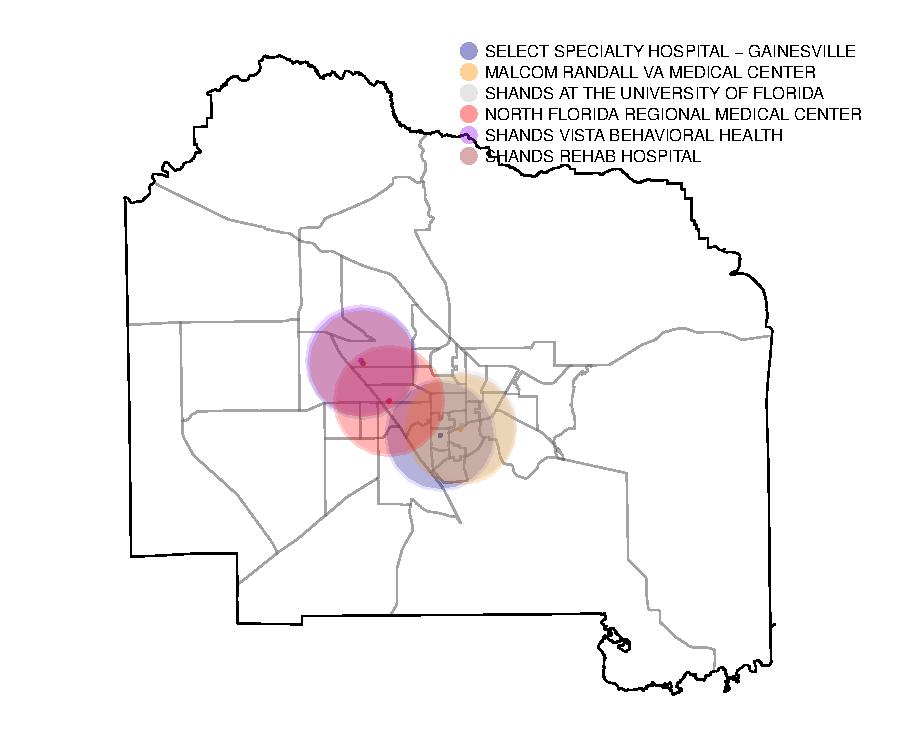
\includegraphics{hw3_R_joe_brew-014}
\end{center}

\end{document}
